\section{Fast Frontier Detector}
% \begin{frame}<beamer>
% \frametitle{Outline}
% \tableofcontents[currentsection,currentsubsection]
% \end{frame}
\subsection*{Background and Outline}

\begin{frame}
\frametitle{\FFD: Fast Frontier Detector}
\begin{itemize}
  %\item The reason lies within the characteristics of new frontiers
%  \item Insights: 
%  	\begin{itemize}
%	  \item New frontiers are never contained within known regions
%	  \item New frontiers are never wholly within unknown regions   
%	\end{itemize} \pause
   \item  Scanning all known regions is definitely unnecessary
 	\begin{itemize} 
 	  \item and not time-efficient
     \end{itemize} \pause
  \item Avoid searching both known and unknown regions
  	\begin{itemize}
  		\item Only process new laser readings
    \end{itemize}
  
\end{itemize}
\end{frame}

\begin{frame}
\frametitle{\FFD Outline}
\begin{enumerate}
  \item Sorting Range Readings
  \item Building Contour of Range Readings  
  \item Detecting New Frontiers
  \item Maintaining Previously Detected Frontiers
   
\end{enumerate}
\end{frame}

\subsection*{Sorting}

\begin{frame}
\label{frame:FFD_Sorting}
\frametitle{Sorting}
\begin{itemize}
  \item Most laser sensors return readings that are already sorted
  	\begin{itemize}
  	  \item Points that are sorted according to polar angle
  	  \item The robot as center
  	\end{itemize}
  \item However, if this is not the case, we can sort them efficiently  
\end{itemize}

\hyperlink{frame:Sorting}{\beamergotobutton{Sorting in details}}

\end{frame}

\begin{frame}
\frametitle{Sorting}
	\begin{figure}
	 \centering
	 \includegraphics<+>[width=0.85\columnwidth,keepaspectratio]{images/sorting_1.JPG}
	 \includegraphics<+>[width=0.85\columnwidth,keepaspectratio]{images/sorting_2.JPG}
	 \includegraphics<+>[width=0.85\columnwidth,keepaspectratio]{images/sorting_3.JPG}
	 \includegraphics<+>[width=0.85\columnwidth,keepaspectratio]{images/sorting_full_points.JPG}
	\end{figure}
\end{frame}



\subsection*{Contour}

\begin{frame}
\frametitle{Contour}
\begin{itemize}
  \item \textbf{Input}: sorted set of points 
  \item \textbf{Output}: a contour that is built from the laser readings set
  %A The desired output is a set of
  %segments that connects The output is a
  %contour built from the sorted laser readings
  \begin{itemize}
    \item The line that connects each two adjacent points from the set
  \end{itemize} 
  \item Calculate the points that lie between each adjacent laser readings
  	
    	\item We use \emph{Bresenham's line algorithm}
		[Bresenham, 1965]
  \item The desired contour contains all the points mentioned above
\end{itemize} 
\end{frame}

% \begin{frame}
% \frametitle{Contour}
% \begin{alertblock}{Problem}
% 	We need the algorithm to be fast and robust against rounding errors
% \end{alertblock} \pause
% \begin{block}{Solution}
% 	We use \emph{Bresenham's line algorithm}
% 	[Bresenham, 1965]%\citep{bresenham2010algorithm}
% \end{block}
% \end{frame}

\begin{frame}
\frametitle{Contour}
	\begin{figure}
	 \centering
	 \includegraphics<+>[width=0.85\columnwidth,keepaspectratio]{images/sorting_full_points.JPG}
	 \includegraphics<+>[width=0.85\columnwidth,keepaspectratio]{images/contour_vectors.JPG}\transfade%\transdissolve
	 \includegraphics<+>[width=0.85\columnwidth,keepaspectratio]{images/contour.JPG}\transfade
	\end{figure}
\end{frame}



\subsection*{Detection}
\begin{frame}
\frametitle{Detecting New Frontiers}
\begin{itemize}
  \item We scan the calculated contour from previous step 
  \item Each point is compared with its (already scanned) predecessor \pause
  \item Four possible cases: 
  	\begin{itemize}
  	  \item Scanned point is not a frontier cell 
  	  \item Scanned point is a frontier cell but its predecessor is not 
  	  \item Both scanned point and its predecessor are frontier points 
  	  \item Scanned point is not a frontier cell but its predecessor is 
  	\end{itemize}  
  %\item Full details can be found in the paper
\end{itemize}
\end{frame}

\subsection*{Maintenance}
\begin{frame}
\frametitle{Maintenance: Motivation}
\begin{itemize}
  \item \FFD gains its speed by only processing the laser readings
  	\begin{itemize}
	  \item rather than entire regions of the map
	\end{itemize}
  \item Robot navigates towards one detected frontier
  \item Other detected frontiers are stored for future usage
  \item Problems:
  \begin{itemize}
    \item Other detected frontiers are not updated during navigation
    \item Avoid detection of frontiers in already visited regions 
  \end{itemize}
  %\item Previously detected frontiers are not updated during navigation 
  %\item Only the frontier that the robot is headed to
\end{itemize} 

% \begin{alertblock}{Problem}
% \FFD is able to detect only \emph{new} frontiers in each execution
% \end{alertblock} 
% 
% \pause
% \begin{block}{Solution}
% Maintenance of frontiers which are not covered in the sensors range
% \end{block}
\end{frame}


% \begin{frame}
% \frametitle{Maintenance: Motivation}
% \begin{itemize}
% %   \item \FFD maintains previously detected frontiers
% %   	\begin{itemize}
% %   	  \item in order to get complete information about frontiers
% %   	\end{itemize} 
% %   \item Joining together new detected and previously detected
% %   frontiers
% %   \item Instead of processing the map, process laser readings directly
% % 	\begin{itemize}
% % 	  \item must run with every new laser reading
% % 	\end{itemize} 
%   \item Maintenance has to deal with:
%   	\begin{itemize}
%   	  \item Elimination of previously no-longer detected frontiers
%   	  \item Avoiding re-detection of same frontier
% %  	  \item Storing new detected frontiers
%   	\end{itemize}
% \end{itemize}
% \end{frame}

\begin{frame}
\frametitle{Maintenance 1: Eliminating Previously Detected Frontiers}
\begin{itemize}
  \item Points which are no longer in frontiers have to be eliminated
  \item \emph{Active Area}: blocking rectangle constructed from laser
  readings
  \item If a frontier is to be eliminated, it must lie inside the active
  area
  	\begin{itemize}
  	  \item it contains regions that are covered by the robot's sensors
    \end{itemize} 
  \item \FFD scans each point that lies inside the \emph{Active Area}
  	\begin{itemize}
  	  \item Quickly checks if a point belongs to a previously detected frontier
  	  %Checking if a point is previously belonged to a frontier is fast
  	  %\item Full details can be found in the paper
  	\end{itemize} 
\end{itemize}

\begin{figure}
	 \centering
	 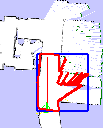
\includegraphics[angle=90,width=0.25\columnwidth,keepaspectratio]{images/active_area1}
\end{figure}
\end{frame}


\begin{frame} 
\frametitle{Maintenance 2: Avoiding Re-detection of Same Frontier}

\begin{columns}
\begin{column}{0.5\textwidth}
	\begin{alertblock}{Problem}
	\FFD might wrongly detect a new frontier in an already scanned area
	\end{alertblock} 
	\begin{figure}
		 \centering
		 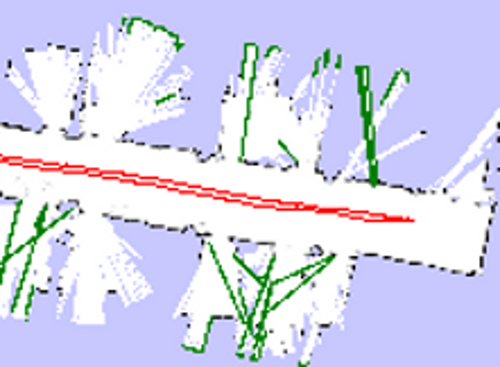
\includegraphics[width=0.7\columnwidth,keepaspectratio]{images/redetecting_bad_example}
	\end{figure}
\end{column}
\begin{column}{0.5\textwidth}
	\begin{block}{Solution}
	\FFD distinguishes between laser readings in different time frames
	\end{block} 
	\begin{figure}
		 \centering 
		 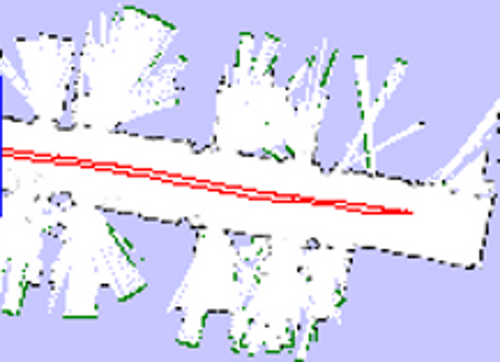
\includegraphics[width=0.7\columnwidth,keepaspectratio,trim = 4pt 0 0 0,
		 clip]{images/redetecting_good_example}
		\end{figure}
	\end{column}
\end{columns}

%\vfill Full details can be found in the paper
\end{frame}


\begin{frame}
\frametitle{\FFD: Summary}
\begin{itemize}
  \item \FFD has to run in the background persistently
  	\begin{itemize}
  	  \item In contrast to other approaches that are executed in a certain time
  	\end{itemize} %\pause 
  \item \FFD requires robustness against map orientation changes
  	\begin{itemize}
  	  \item caused by loop-closures %\pause
%   	  \item In \emph{Particle Filter} based systems, active particle might
%   	  be change
%   	  \begin{itemize}
%   	    \item Particles do not share maps
%   	    \item previously detected frontiers cannot be easily maintained
%   	  \end{itemize} 
%   	  \pause
%   	  \item In \emph{EKF} based systems, the situation is different
% 	  	  \begin{itemize}
% 	  	    \item Only one map is updated
% 	  	    \item Information about changing map orientation is available
% 	  	    \item Therefore, frontier data can be stored within a map
% 	  	  \end{itemize}
  	\end{itemize} 
 \end{itemize} 
\end{frame}

\begin{frame}
\label{frame:ffd_sound_complete}
\frametitle{Correctness of \FFD}
\begin{itemize}
  \item \FFD is complete
  \begin{itemize}
    \item Assume $f$ is a frontier point 
    \item Lemma and Theorem: \FFD will mark $f$ as a frontier point
  	\item \hyperlink{frame:ffd_complete}{\beamergotobutton{Proof in Details}}
  \end{itemize}
  \item \FFD is sound 
  \begin{itemize}
    \item Assume $\hat{f}$ is not a frontier point 
    \item Theorem: \FFD will not mark $f$ as a frontier point
  	\item \hyperlink{frame:ffd_sound}{\beamergotobutton{Proof in Details}}
  \end{itemize}
\end{itemize}
\end{frame}

